\documentclass[en]{./../../common/SurferDesc}%%%%%%%%%%%%%%%%%%%%%%%%%%%%%%%%%%%%%%%%%%%%%%%%%%%%%%%%%%%%%%%%%%%%%%%
%
% The document starts here:
%
\begin{document}
\footnotesize
% Weltrekordfl�chen

%%% 1.Tafel

%%%%%%%%%%%%%%%%%%%%%%%%%%%%%

\begin{surferPage}
  \begin{surferTitle}The Cayley Cubic\end{surferTitle}  \\
   This cubic surface (surface of degree $3$) is also contained in the
    gallery on simple surfaces. 
    Altogether, it has four double cone singularities.
    It is named after Arthur Cayley who did a lot of research on cubics
    in the $19$th century.
    
     However, it was Ludwig Schl�fli who first classified these surfaces in 1863 in
    a systematic way with respect to the possible singularities on them.
    E.g., in his article one can read why there cannot be more than $4$
    singular points on one cubic surface.
    This yields: $\mu(3)=4$. 
    
    Around 1900, Felix Klein studied the possible shapes of real cubic surfaces; 
    his idea was to answer this question starting from the Cayley Cubic by
    means of small deformations:
    By expanding double cone singularities, disconnecting or merging parts,
    he was actually able to find all possible shapes; here are a few of them: 
    \vspace{0.3cm}
     \begin{center}
      \vspace{-0.2cm}
      \begin{tabular}{@{}c@{\ }c@{\ }c@{\ }c@{}}
        \begin{tabular}{@{}c@{}}
          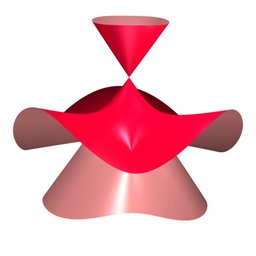
\includegraphics[width=1.35cm]{./../../common/images/cayley_cubic_0}
        \end{tabular}
        &
        \begin{tabular}{@{}c@{}}
          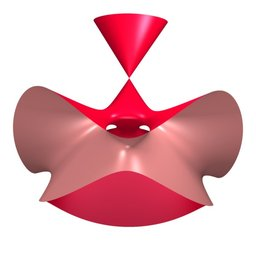
\includegraphics[width=1.35cm]{./../../common/images/cayley_cubic_1}
        \end{tabular}
        &
        \begin{tabular}{@{}c@{}}
          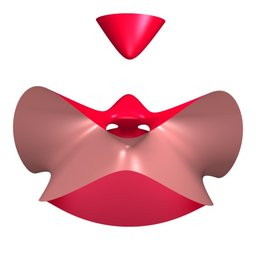
\includegraphics[width=1.35cm]{./../../common/images/cayley_cubic_2}
        \end{tabular}
        &
        \begin{tabular}{@{}c@{}}
          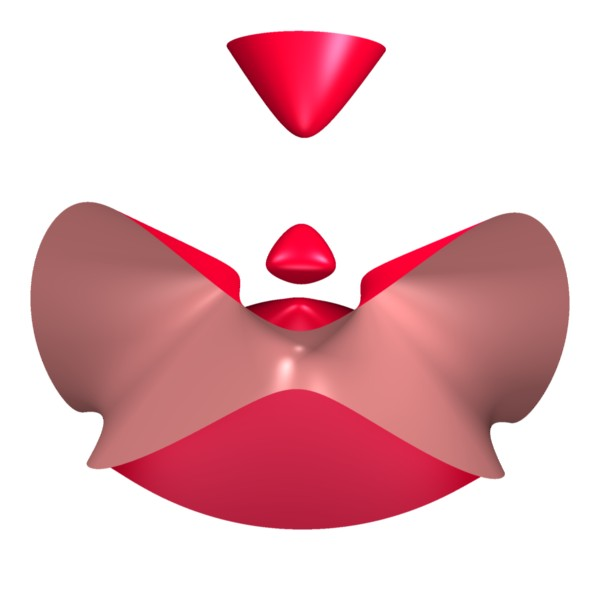
\includegraphics[width=1.35cm]{./../../common/images/cayley_cubic_3}
        \end{tabular}
      \end{tabular}
    \end{center}

  \begin{surferText}
     \end{surferText}
\end{surferPage}

%%%%%%%%%%%%%%%%%%%%%



\end{document}
%
% end of the document.
%
%%%%%%%%%%%%%%%%%%%%%%%%%%%%%%%%%%%%%%%%%%%%%%%%%%%%%%%%%%%%%%%%%%%%%%%
